\begin{multicols}{3}[\section{Formatvorlage}]

\rhead{Alexander Härtel}
\lfoot{10.04.2016}

\newrefsegment

\begin{tabular}{p{2,1 cm}p{2.7 cm}}
\textbf{Steckbrief}& \\
\end{tabular}
\rowcolors{1}{\topicolor!20}{}
\begin{tabular}{p{2,1 cm}p{2.7 cm}}
      Einsatz seit & 20.03.2016\\
      Frequenz"-bereich  & \SI{2500}{\giga\hertz}\\
      Datenrate & \SI{777}{bit/s}\\
      Verbreitung & Weltweit, Scientific Community\\
      Reichweite & \SI{500}{\kilo\metre}\\
\end{tabular}
\par
%Source http://www.fh-bingen.de/fileadmin/user_upload/Lehrende/Kilsch_Dieter/internet/projekte/TedoSchStiUnits.pdf -> Seite 9 findet ihr alle verwendbaren Einheiten, wie:
%\SI{Zahl}{\mega\hertz} oder \SI{Zahl}{\mili\metre}
%Ich weiß ehrlich gesagt nicht welche Einheiten ihr im Text genau braucht, aber in dem Dokument und mit obigen Beispiel sollte es umsetzbar ein.
\subsection*{Überblick}
Diese Vorlage ist der erste vollständige funktionierende Entwurf für die von euch zu verfassenden Kapitel. Es besteht essentiell aus 4 Dateien:
\begin{itemize}
	\item Header
	\item Hauptdokument
	\item Vorlage
	\item BibTex-Dokument
\end{itemize}

Für diejenigen, die \LaTeX~noch nicht kennen, gibt es im nächsten Abschnitt eine kurze Erklärung. Euer Fokus wird auf dem Vorlagendokument und seiner BibTex liegen (Unter Kapitel/EuerTitel). Dort müsst ihr euren Text mit diesem hier austauschen und einige Formatierungen bei zum Beispiel Bildern oder Einheiten beachten. In der BibTex-Datei haltet ihr eure Quellen fest auf die ihr im Text referenziert. 

Solltet ihr eine \LaTeX-Umgebung haben, könnt ihr über das Hauptdokument eure Änderungen testen, aber seit gewarnt: Ihr müsst einige Pakete installieren, um dies durchzuführen.

\subsection*{Technische Erläuterungen}
Über im Header angeforderte Pakete und gesetzte Definitionen wird das gesamte Dokument so eingestellt, das es aussieht, wie gerade jetzt. Zur Umwandlung von \LaTeX~ins Pdf-Format könnt ihr zum Beispiel das Softwarepaket MikTex benutzen. Dort ist das Programm TeXworks enthalten mit dem ich dieses Dokument erstellt habe. Auf einschlägigen Seiten oder bei anderen Nutzern könnt ihr euch mehr darüber informieren, insofern ihr das wollt. 

Im Grunde fungiert die Umgebung, die ihr installieren müsst, wie nichts anderes als eine Entwicklungsumgebung, wie zum Beispiel Eclipse. Ihr stellt ein wie es umgewandelt werden soll und der Rest passiert im Hintergrund. Beim Kompilieren werden euch unterschiedliche Einstellungen geboten. Ich verwende \enquote{pdfLatex + MakeIndex + BibTex} (Auch wenn genau genommen kein Index verwendet wird. TeXworks ignoriert diesen Schritt dann.). Alternativ und wahrscheinlich sogar lehrreicher ist das Kompilieren über BibTex und anschließend über pdfLatex. 

Was passiert? Über die Einstellung BibTex bekommt TeXworks die Anweisung für das Hauptdokument alle eingebundenen BibTex-Dateien, hier zu unter Gremien mehr, zusammenzutragen. Es entstehen mehrere Dateien und am Ende eine mit dem Titel \enquote{Hauptdokument-blx.bib}. Bei pdfLatex wird diese Datei mit herangezogen, wenn ihr im Text zitiert und auf die Quelle referenziert. Beispiele sind im nachfolgenden Text eingestreut. 

\subsection*{Einsatz}
In Zeile 3 kommt in die geschweifte Klammer hinter \enquote{section} euer Titel des Themas. In der darauffolgenden Zeile ersetzt ihr den Autor und dann das Bearbeitungsdatum.
\begin{Figure}

\includegraphics[width=\linewidth]{Kapitel/Vorlage/Grafiken/bild2_dhbw.jpg}
\captionof{figure}{Vorlesungssaal der DHBW Mannheim~\cite{vorlage.7}}
\label{fig:vorlage.vorlesungssaal}
\end{Figure}
Das Bild \ref{fig:vorlage.vorlesungssaal} hat eigentlich keinen Bezug zu dem ganzen Text. Erzeugt jedoch einen ordentlichen und schönen Einblick in einen Vorlesungssaal, den man zweimal im Jahr betritt.

Mit Zeile 9 befindet ihr euch im Steckbrief. In \LaTeX-Tabellen werden Spalten in der Regel durch \enquote{\&} getrennt und Zeilen durch Doppelslash beendet. Interessant sind hier die Einheiten, die ihr verwendet müsst. Ich habe einige Beispiele auskommentiert (Alles hinter einem \enquote{\%} ist ein ordinärer Kommentar). Sollte eure gewünschte Einheit nicht dabei sein, fragt bei uns nach oder informiert euch über das Paket \enquote{siunitx}~\cite{vorlage.1}.

Nun folgen die einzelnen Abschnitte. Diese Abschnitte sind hier durch \enquote{subsection} gekennzeichnet. Insofern du keine Anführungszeichen, \%, \&, Einheiten oder andere Funktionszeichen von Latex brauchst, musst du einfach nur den Text ersetzten. Den Text kannst durch eine freie Zeile in Absätze separieren. 

Brauchst du wider erwartend doch derlei Zeichen, musst du ihn beim Einfügen entsprechend überarbeiten. Dabei sollte dieser Beispieltext als guter Leitfaden dienen.

\subsubsection*{Ich will meinen Text weiter unterteilen!}
Das ist natürlich möglich. Dafür müsst ihr ein Statement der Form \enquote{\textbackslash subsubsection*\{Titel der Unterüberschrift\}} verwenden. Macht das bitte nicht beim \textit{Ausblick!}

\subsubsection*{Bilder?}
\begin{Figure}

\includegraphics[width=\linewidth]{Kapitel/Vorlage/Grafiken/sg_ft_zemath.png}
\captionof{figure}{Titelbild der Zemath der DHBW~\cite{vorlage.8}}
\label{fig:vorlage.zemath}
\end{Figure}
Auch zu dem Bild \ref{fig:vorlage.zemath} lässt sich nur sagen, das es eigentlich nichts mit dem Text zu tun hat. Es ist ein Aushängeschild einer Organisation, die uns Studenten helfen soll.

Bilder sollen einen Text auflockern und Informationen komprimieren sagt man und für das Einfügen braucht man ein Statement, das ihr zweimal in diesem Text begutachten könnt. 

Habt ihr ein Bild, speichert ihr es unter eurem Grafikordner. Bedenkt dabei das der Order \enquote{EuerTitel} und die Bilddatei keine Leerzeichen, ä, ö, ü oder andere Absurditäten enthalten darf. \LaTeX~reagiert da allergisch drauf und verschluckt sich beim Kompilieren, weil der den Pfad nicht entlang laufen kann. Die Basissprache ist halt doch schon etwas älter.

So nun habt ihr das Bild und sicherlich auch noch die Quelle offen. Die Quelle speichert ihr in euer BibTex-Datei als Online-Eintrag. Das war der Sinnvollste auf den ersten Blick. Kopiert euch die obige Bildumgebung \enquote{\textbackslash begin\{Figure\} bis \textbackslash end\{Figure\}} und passt den Pfad an. Beim \enquote{captionof} verändert ihr das zweite Paar geschweifte Klammern mit einer kurzen aber klaren Beschreibung, die dem Leser alles gibt, was er über das Bild wissen muss, um es zu verstehen. 

Noch bevor ihr das Ende der geschweiften Klammer erreicht fügt ihr die Referenz auf die Quelle ein. Die Tilde sorgt dafür das \LaTeX~den Text an dieser Stelle nicht unterbricht und genau ein Leerzeichen setzt. 

Zu guter Letzt solltet ihr innerhalb des Textes auch auf das Bild verweisen. Dafür definiert ihr ein Label. Es sollte wie folgt aussehen: \enquote{fig:euertitel.wasfüreucheindeutiges}

\enquote{fig:} steht für nichts anderes als Figure und gehört zu den \LaTeX~Best Practices. Damit der Verweis innerhalb des kompletten Dokumentes eindeutig bleibt, folgt euer Titel der mit einem Punkt etwas für euch Wiedererkennbares anschließt. So ist es möglich im Text auf ein Bild \enquote{\textbackslash ref\{fig:euertitel.wasfüreucheindeutiges\}} zu verweisen. 

Im nächsten Abschnitt gehen ich etwas genauer auf BibTex und die Referenzierung im Text ein.

\subsection*{Anbieter und Gremien}
\textbf{Bibetex!} 

(Mit \enquote{\textbackslash textbf\{Mein Text\}} geht übrigens fette Schrift. Mit \enquote{textit} würdet ihr kursiv erreichen)

Unter \enquote{./Kapitel/Vorlage/} solltet ihr eine Datei mit dem Namen \enquote{vorlageBib.bib} finden. In ihr sind einige Beispiele angegeben, wie ihr eure Quellen angeben solltet. Eine gekürzte Kopie der Datei mit dem Namen \enquote{EuerTitelBib.bib} findet ihr auf der Ebene eures Textdokumentes (./Kapitel/EuerTitel/EuerTitel.tex).

Ein Eintrag beginnt mit @ und der Kategorie, in die die Quelle passt. In geschweiften Klammern folgen Komma-separiert i.d.R. diese Angaben~\cite{vorlage.2}:

\begin{itemize}
	\item Referenz für den Text
	\item Autor 
	\item Titel
	\item Veröffentlichungsjahr
	\item gegebenenfalls URL
	\item gegebenenfalls ISBN
\end{itemize}

\end{multicols}
\newpage
\section*{Historische Entwicklung}
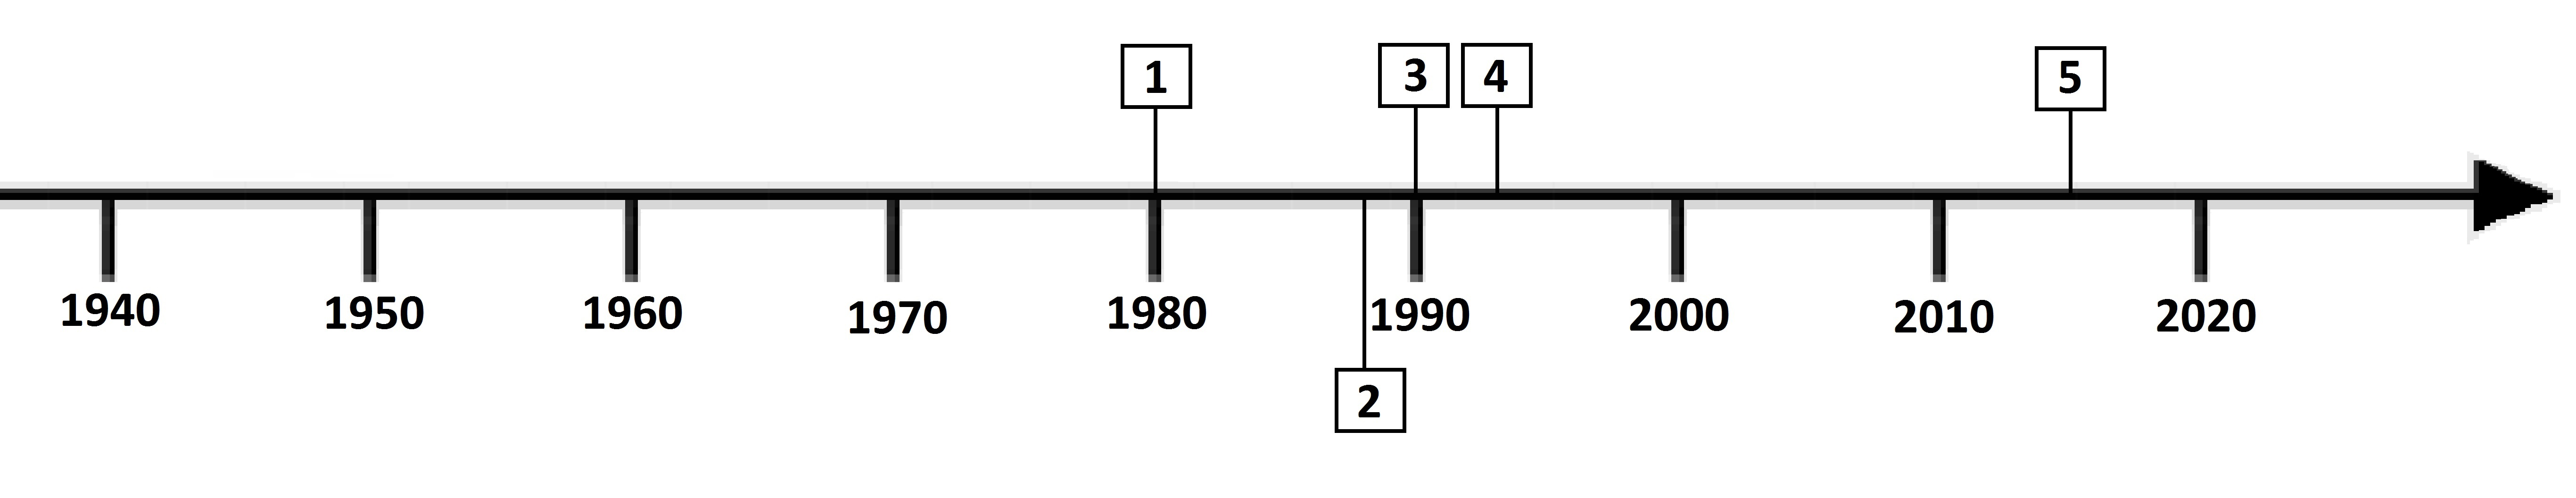
\includegraphics[width=\textwidth]{Kapitel/Vorlage/Grafiken/Zeitstrahl}
\par
\noindent
\rowcolors{2}{}{\topicolor!20}
\begin{tabular}{p{0.5 cm}p{1.5 cm}p{15.55 cm}}
	Nr. & Datum & Entwicklungsschritte~\cite{vorlage.3}\\
	1 & Anfang 80er & Leslie Lamp entwickelt auf \TeX aufbauend eine Sammlung von \TeX-Makros für den durchschnittlichen Anwender.\\
	2 & 1989 & Beginn der Entwicklung der aktuellen Version \LaTeX 2.\\
	3 & 1990 & Ende von Leslie Lamp's \LaTeX-Entwicklung mit Version 2.09.\\
	4 & Mitte 90er  & \LaTeX wird am weitesten verbreitete Methode \TeX zu verwenden.\\
	5 & 20.03.2016 & Beginn der Entwicklung dieser Vorlage in \LaTeX.\\
\end{tabular}
\par
\begin{multicols}{3}

Die Referenz für den Text ist so aufgebaut, wie beim Label für Bilder. Erst kommt euer Titel und mit einem Punkt separiert folgt eine eindeutige Wiedererkennung.

Damit die BibTex-Datei durch die Umgebung gefunden werden kann, müsst ihr in der \enquote{Header.tex} eine Ergänzung durchführen. Aktuell ab Zeile 60 werden dort die BibTex-Dateien eingebunden. Hier müsst ihr den existenten Eintrag ändern zu \enquote{addbibresource\{./Kapitel/EuerTitel/EuerTitelBib\}}. Wichtig ist das ihr nicht \enquote{.bib} mit dazu schreibt. BibTex weiß was es bei diesem Kommando erwartet und mag es nicht zweimal darauf hingewiesen zu werden. Wenn doch läuft es in einen Fehler und ignoriert die Datei.

Ähnliches Prozedere müsst ihr im Hauptdokument (Hauptdokument.tex) vornehmen. In der Zeile \enquote{input\{Kapitel/Vorlage/Vorlage.tex\}} müsst ihr den String \enquote{Vorlage/Vorlage.tex} durch \enquote{EurenTitel/EurenTitel.tex} ersetzen. 

\subsection*{Ausblick}
Mir ist bewusst, dass es denjenigen, die noch keine Erfahrung mit \LaTeX~haben, es erstmal ungewohnt vorkommt, aber ihr solltet euch an diesem Beispieldokument entlang hangeln können. Fragen können jederzeit an die Redaktions-Adresse gerichtet werden.

Zur Abklärung eventuell offener Fragen ist auf der Dropbox demnächst auch ein FAQ abgelegt, das ihr zur Rate ziehen sollt, bevor ihr mich in der Pause oder per Mail ausfragt. (Bildquelle:~\cite{vorlage.8})

\printbibliography[segment=1,heading=subbibliography]
\end{multicols}
\begin{Figure}

\includegraphics[width=\linewidth]{Kapitel/Vorlage/Grafiken/sg_ft_zemath.png}
\captionof{figure}{Titelbild der Zemath der DHBW}
\end{Figure}

\newpage
